\documentclass[10pt]{article}

\usepackage{amsmath}
\usepackage{amssymb}
\usepackage{hyperref}
\usepackage{todonotes}
% \usepackage{biblatex}
\usepackage[margin=1.5in]{geometry}
\usepackage{tikz}
\usetikzlibrary{positioning}

\hypersetup{pdftex,colorlinks=true,allcolors=blue}
\usepackage{hypcap}


\begin{document}

\title{Abstract Interpretation}
\author{William Schultz}
\date{\today}

\maketitle


If we want to analyze the behavior of a program, we typically perform some kind of \textit{abstraction}. That is, we approximate the concrete semantics of the program in some way that is sufficient for analysis. \textit{Abstract interpretation} provides a formal framework for defining and performing these types of program abstractions.

An \textit{abstraction domain} is defined as follows: 
\begin{itemize}
    \item $C$ is a \textit{concrete domain} i.e., a set of elements with an associated partial order $\leq$.
    \item $A$ is an \textit{abstract domain} with associated partial order $\sqsubseteq$ (elements of $A$ form a lattice).
\end{itemize}
We then define mappings between these two sets:
\begin{itemize}
    \item $\gamma : A \rightarrow C$: A \textbf{concretization function} that maps abstract values to sets of concrete elements.
    \item $\alpha : C \rightarrow A$: An \textbf{abstraction function} that maps sets of concrete elements to the most precise value in the abstract domain. 
\end{itemize}
where $\alpha$ and $\gamma$ must form a \textit{Galois connection}. That is, they satisfy the following condition
\begin{align*}
    \forall c \in C, \forall a \in A : \alpha(x) \sqsubseteq a \Leftrightarrow c \sqsubseteq \gamma(a) 
\end{align*} 
\begin{center}
    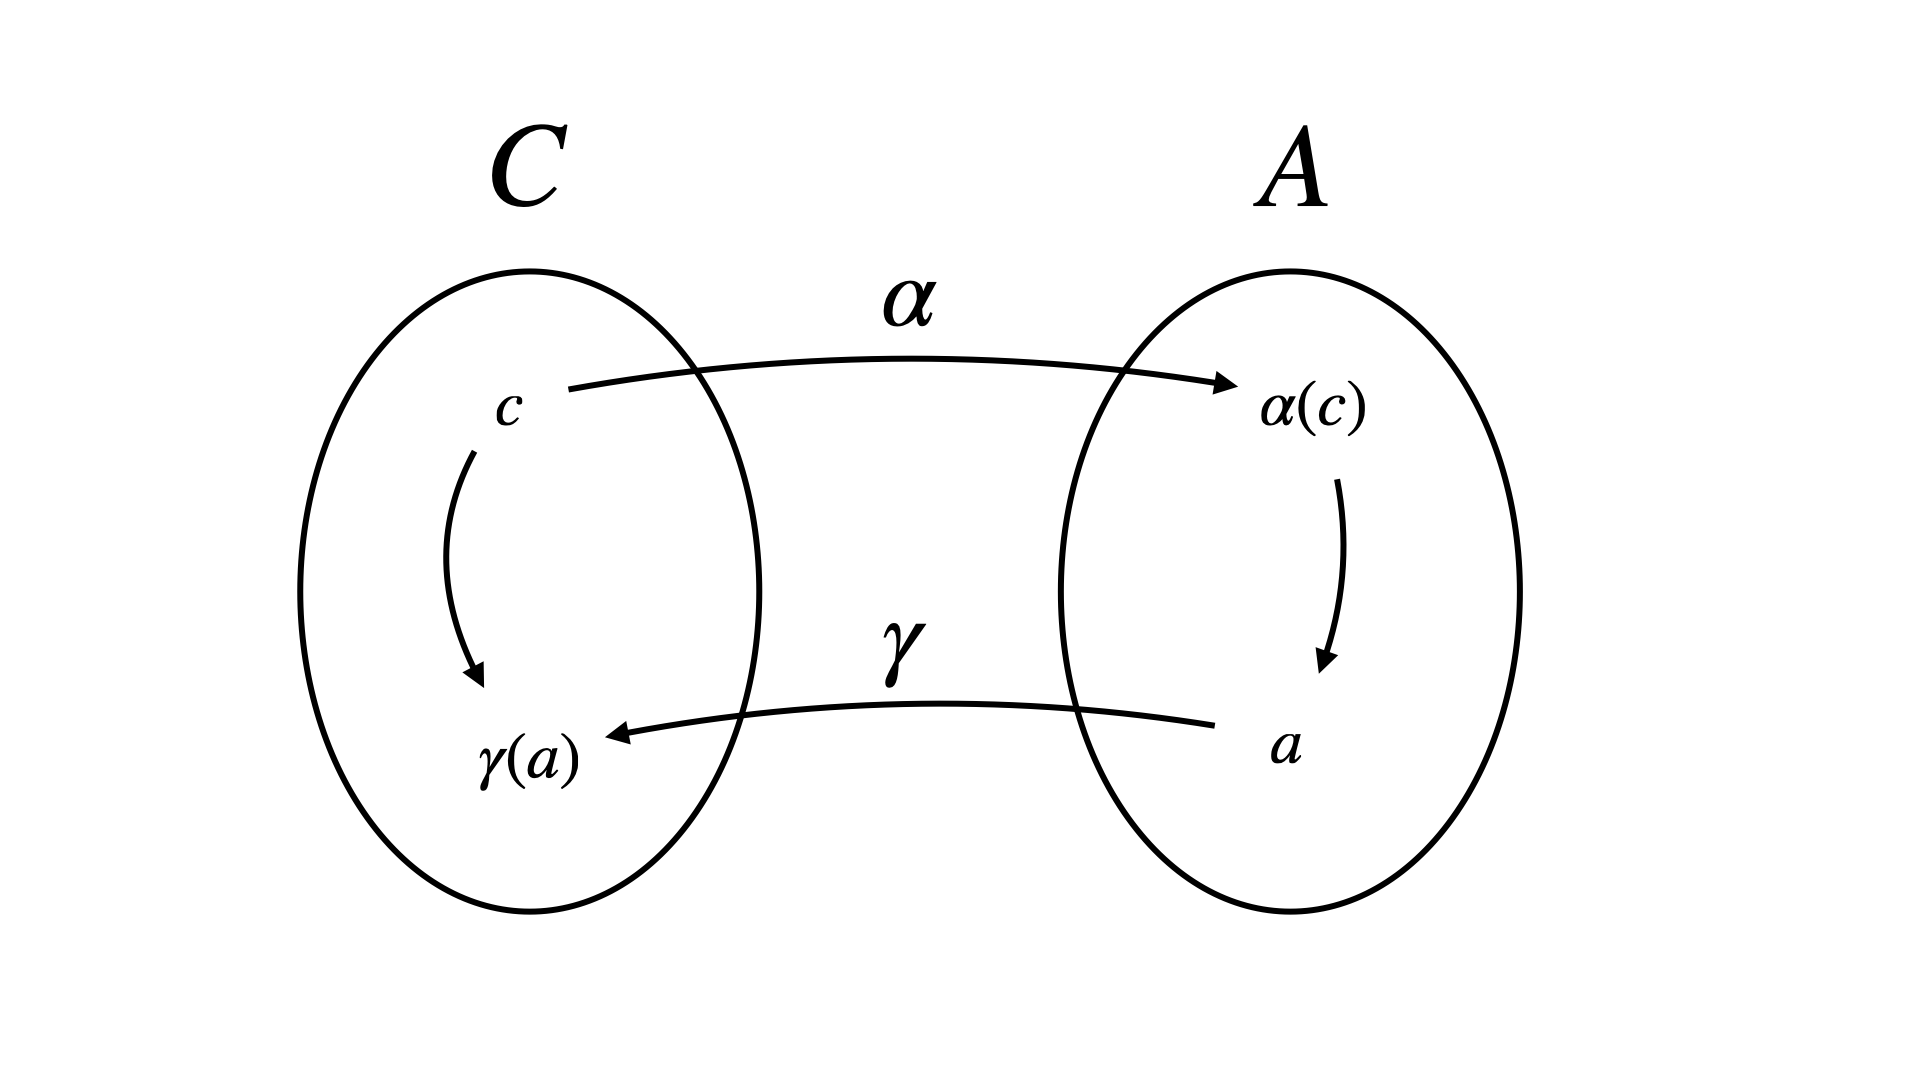
\includegraphics[scale=0.15]{diagrams/diagrams.001.png}
    \textbf{TODO}
\end{center}
Note that a \textit{lattice} $L=(S,\sqsubseteq)$ is a partially ordered set where each pair of elements has a least upper bound (i.e. \textit{join} $\sqcup$) and a greatest lower bound (i.e. \textit{meet}, $\sqcap$).

Intuitively, the above requirements means that the abstraction and concretization functions respect the orderings of $D$ and $A$. That is, if $\alpha(x)$, the abstraction of $x$, is ordered before some other $\hat{x} \in A$, then $x$ should be ordered before $\gamma(\hat{x})$, the concretization of $\hat{x}$.

% Note that we also have \textit{abstract transformers}, which are functions $T: A \rightarrow A$, and which are \textit{sound} if they respect the over-approximation property i.e., if an original abstract element $d$ is an overapproximation of its concretization, then after applying the transformer to $d$, it will remain an overapproximation of the concretization of the transformed value. TODO: Make this clearer. 


\end{document}